\renewcommand*{\thefootnote}{\arabic{footnote}}

\mbox{}\\
\vspace{8cm}

\section{The burden of bacterial pathogens}

Science has made great strides in understanding the ubiquity and complexity of microorganisms since the first observations by Antonie van Leeuwenhoek in the 17th century. The inquisitiveness of the scientific method revealed a myriad of microscopic shapes and interactions that play a pivotal role in global ecosystems and impact nearly every aspect of human activity, from beneficial applications in the food production industry to the detrimental effects on human and animal health. The latter association was discovered by Robert Koch in the 19th century, whose experiments enabled to identify bacteria as causative agents of deadly infectious diseases. Koch’s contributions, along with those of other prominent scientists such as Louis Paster, established the fields of microbiology and bacteriology. The extensive research that followed revealed the enormous diversity of bacterial species, which today constitute one of the three domains of life established by Carl Woese in 1990 \cite{woese_towards_1990, woese_bacterial_1987}.
Bacteria are single-celled organisms that lack a nuclear membrane and divide by binary fission. Superficially, bacteria may appear as simple forms of life. In reality, life is rarely simple and bacterial species exhibit tremendous diversity. This diversity arises from the selective forces that shape bacterial evolution towards the path that maximizes competitiveness in each habitat, giving rise to varied morphologies (e.g., cocci, rods, spirilla, filamentous), sizes (from as small as about 0.2 micrometer ($\mu m$) in diameter to more than 700 $\mu m$ in diameter), nutrient preferences (e.g., glucose is a good carbohydrate source for many species, but some species may prefer other sources, such as lactose in the case of lactic acid bacteria) and structures (e.g., differences in cell wall structure between Gram-positive and Gram-negative bacteria).
Small structural differences can cause significant changes in the way bacteria interact with the environment or a host. For example, modifications in penicillin-binding proteins present in the cell wall, to which the antibiotic penicillin binds, consequently weakening the cell wall and leading to cell lysis, can confer reduced susceptibility or resistance to penicillin. The mechanisms through which bacteria develop \ac{AMR} are of great concern to public health. In 2021, 4.71 million deaths were estimated to be associated with bacterial \ac{AMR} \cite{naghavi_global_2024}. Although deaths attributed to \ac{AMR} among children under 5 years of age have been decreasing, deaths among older people have increased, and it is estimated that by 2050 8.22 million deaths may be associated with \ac{AMR}. Reducing the number of deaths related to \ac{AMR} is an important step to reduce the total number of deaths related to infection. A recent study estimated that in 2019 nearly 14 million deaths were infection-related, with 56\% of those deaths associated with only 33 bacterial pathogens (Figure \ref{fig:introduction_figure1}).

\begin{figure*}[!ht]
    \centering
    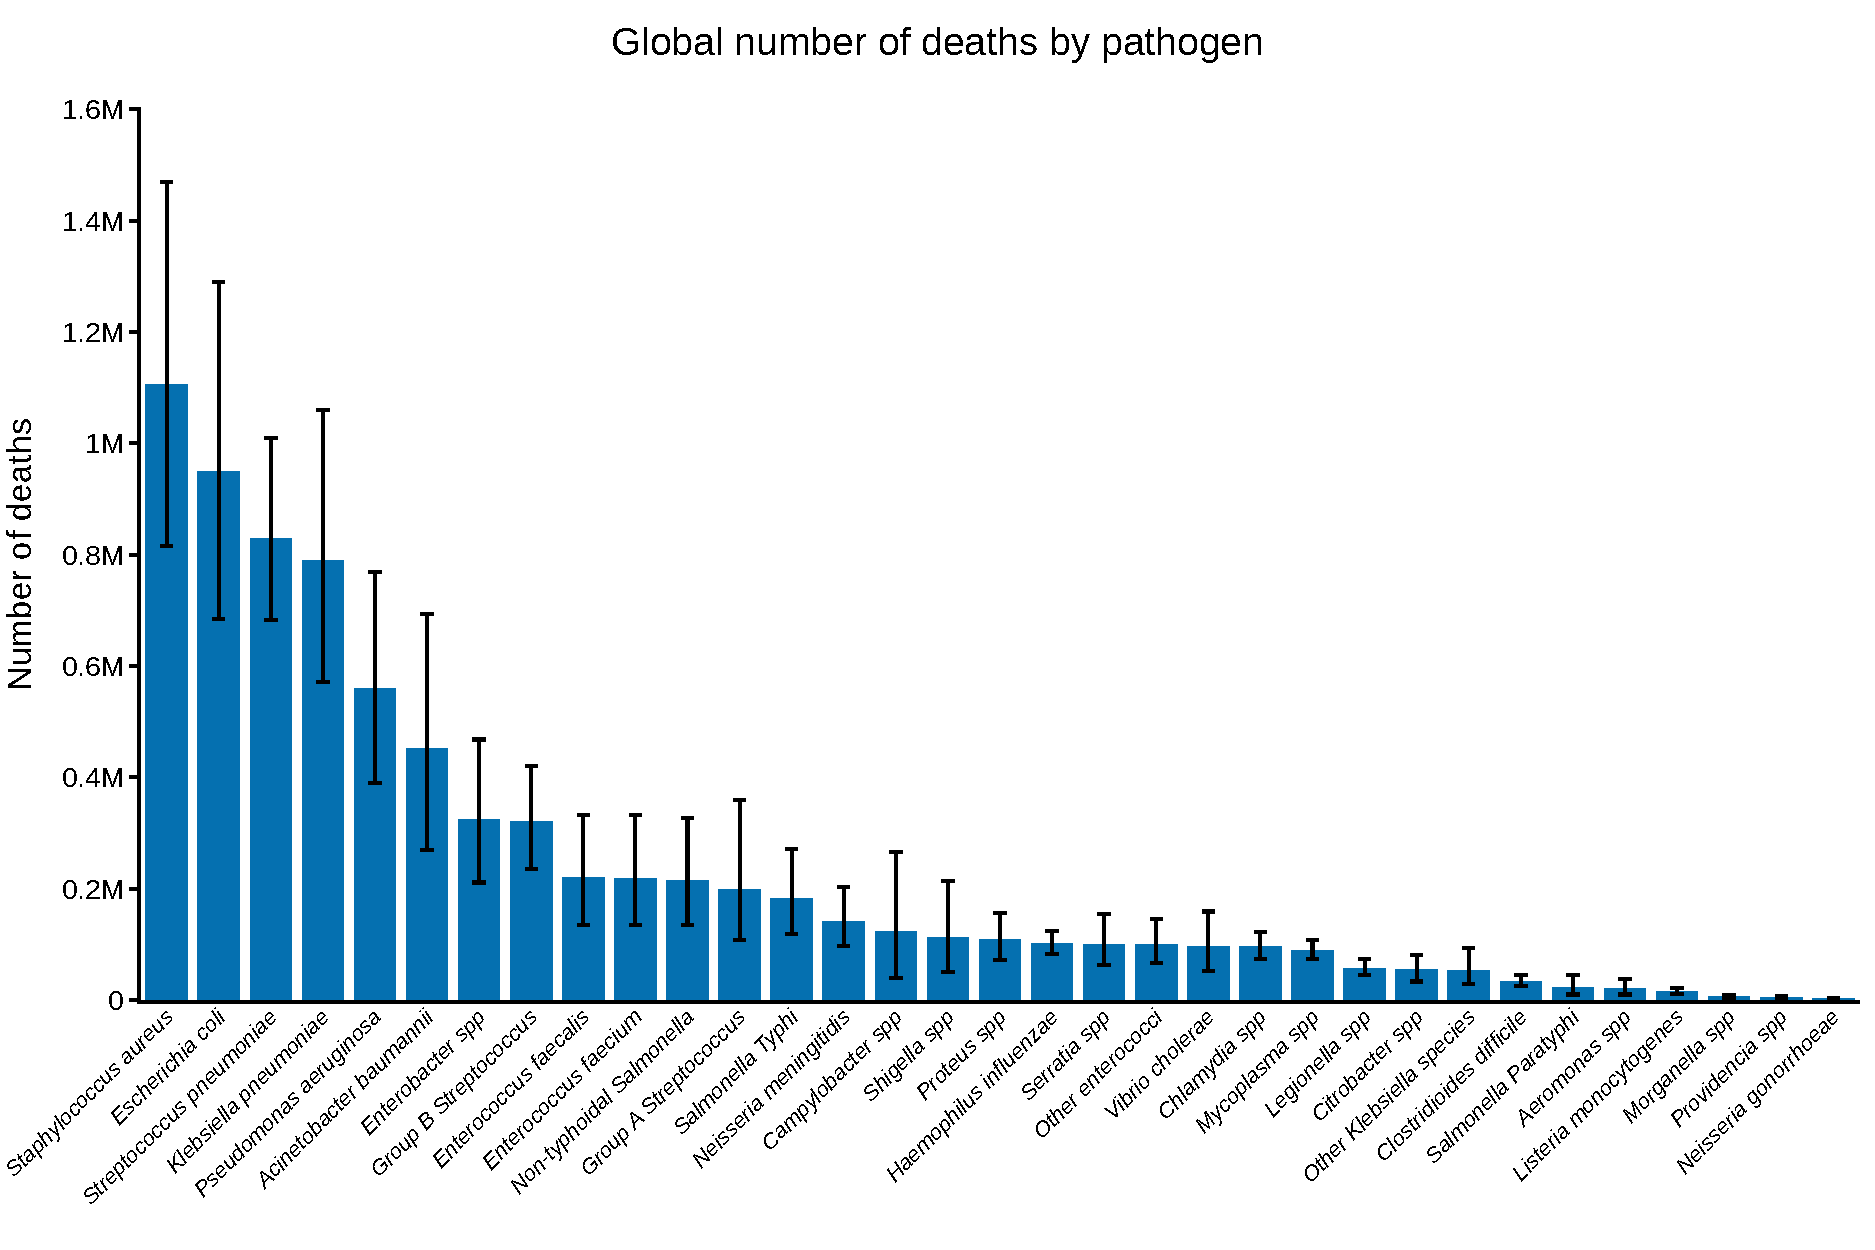
\includegraphics[angle=0,width=\textwidth]{figures/introduction/Figure1.pdf}
    \caption[Global number of deaths, in millions, associated with 33 bacterial pathogens in 2019]{Global number of deaths, in millions, associated with 33 bacterial pathogens in 2019. The error bars represent the 95\% uncertainty intervals. Adapted from \cite{ikuta_global_2022}.}
    \label{fig:introduction_figure1}
\end{figure*}

In the context of global mortality, these estimates put deaths associated with bacterial infections as responsible for at least 14\% of all global deaths \cite{ikuta_global_2022}. Moreover, the top five pathogens were associated with half of all bacterial deaths. These five pathogens are included in the \ac{WHO} \ac{BPPL} updated in 2024 \cite{who_bppl_2024}. The \ac{BPPL} groups 15 families of antibiotic resistant pathogens into priority levels, with the aim of serving as a compass for \ac{RD} and for public health action (Figure \ref{fig:introduction_figure2}). A global concerted effort of public health authorities is of the utmost importance to implement regionally tailored strategies to reduce the burden caused by bacterial infections. The implemented measures should combine infection prevention, vaccination, adequate methods of bacterial characterization and antibiotic usage, as well as promote \ac{RD} aiming to strengthen the resilience of these measures and future preparedness. Although all of these measures must be taken into account to develop effective strategies, the following sections will focus on common techniques used to characterize bacterial pathogens, with increasing emphasis on the application and impact of \ac{HTS} technologies and bioinformatics methods, steering us towards the objectives of this dissertation.

\begin{figure*}[!ht]
    \centering
    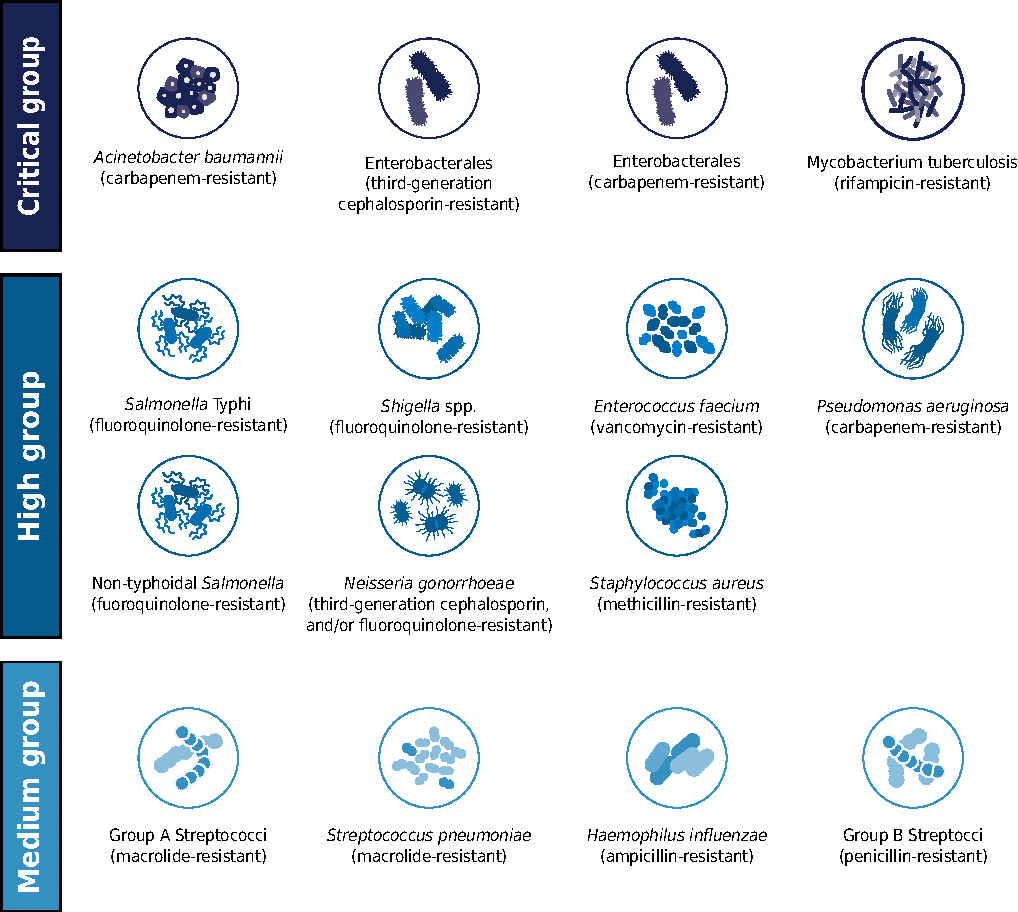
\includegraphics[angle=0,width=\textwidth]{figures/introduction/Figure2.pdf}
    \caption[\ac{WHO} Bacterial Priority Pathogens List, 2024 update]{WHO Bacterial Priority Pathogens List (BPPL), 2024 update. The \ac{BPPL} includes 15 families of \ac{ABR} pathogens, grouped into critical, high and medium categories of priority for \ac{RD} and for public health measures. Adapted from \cite{who_bppl_2024}.}
    \label{fig:introduction_figure2}
\end{figure*}

\section{Bacterial characterization}

The characterization of pathogen strains is essential for the effective management of infected patients and the epidemiology of infectious diseases. Bacterial characterization or typing methodologies can be divided into phenotyping and genotyping \cite{li_bacterial_2009}. The former characterizes bacteria based on phenotypic assays, such as colony morphology on various culture media, biochemical tests, serology, and antibiotic susceptibility. The latter distinguishes bacteria on the basis of their genetic content and has been increasingly adopted to complement or substitute phenotypic assays. Genotyping allows inferring phenotypic characteristics through methods that are less complex and more broadly applicable than classical phenotypic assays, and in many cases has the potential to provide greater resolution. Microbiologists use both approaches to infer specific phenotypic characteristics, such as susceptibility to antimicrobial drugs, allowing to set the best course of action for patient treatment or mitigate the impact of an outbreak. Phenotypic assays rely on the expertise of clinical microbiologists who apply specialized and often species-specific techniques that were developed and optimized over years of research. These techniques involve complex and multi-step protocols that, depending on the bacterial species, can take less than a day or a few days (e.g. rapid-growing bacteria such as \textit{Escherichia coli} \cite{son_growth_2021}), to several weeks (e.g. slow-growing bacteria such as \textit{Mycobacterium tuberculosis} \cite{gordon_microbe_2018}) \cite{didelot_transforming_2012}. The application of \ac{HTS}, in combination with the development of specialized bioinformatics methods, has allowed researchers to reduce sample turnaround time by avoiding specific methodologies in favor of approaches such as \ac{WGS}, which allows to accurately identify the genomic features associated with the phenotypic characteristics of interest from sequence data to provide equivalent results to more laborious and time-consuming lab protocols. Notwithstanding the impact of the latest developments in sequencing technologies and bioinformatics methods, there is still no single method for bacterial characterization that is universally ideal, with each method having to strike a balance between several desired characteristics, such as being applicable to all isolates, highly discriminatory at all levels, generating reproducible results at intra- and inter-laboratory level, while also using modest resources.

\section{Phenotypic methods}

Classical bacteriology methodologies are based on successfully isolating a bacterial pathogen on culture media. Given that different bacterial species may have different growth requirements, microbiologists had to develop a wide repertoire of techniques to account for all the variable requirements. After successfully isolating a pathogen, microbiologists may perform a series of assays to determine, for example, the species of the pathogen and its antimicrobial and virulence profiles (Figure \ref{fig:introduction_figure3}). The culture step varies according to the complexity of a sample. For samples from usually sterile sites, such as cerebrospinal fluid, it may be possible to report all organisms present in the sample and it is simpler to identify the ones that are clinically relevant and should go through further analysis steps. In the case of complex samples, such as faeces, isolating the \textit{micro culprit} may require a more custom approach guided by an educated guess about likely pathogens to select the appropriate media for culture and subsequent tests for a definitive diagnostic.

A correct species identification is highly informative, as it allows to deduce intrinsic characteristics from the body of knowledge and estimate the pathogenic potential, especially in the context of the isolation site. To identify the species of an isolate, microbiologists may use Gram staining, evaluate colony growth and morphology, and perform rapid biochemical tests, such as a bile solubility test, which is used to differentiate \textit{Streptococcus pneumoniae} from other alpha-hemolytic streptococci. Determining the biomolecule profiles of pure suspensions through \ac{MALDI-TOF} mass spectrometry and comparing them with known profiles is also used for rapid and cost-effective species identification, and to identify toxins and study bacterial antibiotic resistance \cite{croxatto_applications_2012, lasch_maldi-tof_2025, alizadeh_maldi-tof_2021, seng_ongoing_2009, idelevich_rapid_2018}.

Following culture and species identification, the determination of the antimicrobial resistance profile is crucial to select an effective treatment for infected patients. Antimicrobial resistance tests are mainly based on inhibition of \textit{in vitro} bacterial growth when exposed to an antibiotic. The efficacy of testing methods, such as disc diffusion and E-TEST, is compared against gold-standard susceptibility-testing systems, such as micro-dilution, to infer \textit{in vivo} efficacy.
The level of susceptibility to a given antibiotic is based on the \ac{MIC} and on the definition of \textit{breakpoints}, which correspond to the antibiotic concentration above which an isolate is considered to be resistant to therapy \cite{didelot_transforming_2012}. \textit{Breakpoints} are defined based on various factors that are not necessarily universally agreed upon, making it difficult to accurately compare and assess the efficacy of susceptibility testing and associate it with clinical outcome. Moreover, it is important to note that the results of susceptibility testing may not translate into similar \textit{in vivo} results, as resistance mechanisms may be more complex and depend on factors not adequately emulated by current susceptibility testing practices \cite{didelot_transforming_2012, hassall_limitations_2024}.

Compared to antimicrobial susceptibility testing, the detection of virulence factors tends to be overlooked when selecting an effective treatment for patients. Nonetheless, knowledge of the virulence profile of pathogens can play an important role when the presence of a virulence factor is known to contribute significantly to pathogenesis and disease severity. For example, toxin-producing strains of \textit{Clostridioides difficile}, the most common cause of nosocomial antibiotic-associated diarrhea \cite{buddle_pathogenicity_2023}, are pathogenic and may require differential treatment. Another example is the \ac{PVL} cytotoxin produced by some \textit{Staphylococcus aureus} strains, which contributes to increased pathogenicity and disease severity, especially when combined with resistance to methicillin, and is associated with community-acquired severe necrotizing pneumonia and necrotic lesions of the skin and subcutaneous tissues \cite{lina_involvement_1999, vandenesch_community-acquired_nodate, tristan_global_nodate, diep_contribution_2008, lee_methicillin-resistant_2018}. In public health, virulence factors are especially important as vaccine targets. For example, the variability of the capsule polysaccharide of \textit{Streptococcus pneumoniae} is detected by serotyping and epidemiologically relevant serotypes are targeted for vaccine development \cite{henrichsen_six_1995, tarrago_identification_2008, silva-costa_adult_2023, musher_remarkable_2022}. Serotyping is a method that uses antisera, which are sera containing antibodies against specific antigens, to identify and classify microorganisms based on their surface antigens. Serotyping provides enough discriminatory power to distinguish different strains of a pathogen, which is essential for public health interventions. Serotyping is a good example of a phenotypic assay that is routinely applied and for which there are sequence-based genotyping alternatives, generally applied after \ac{WGS} to complement laboratory results or to determine the serotype of strains of interest when only sequence data is available. In the case of \textit{S. pneumoniae}, \textit{in silico} serotyping is possible through specialized sequence databases\footnote{\url{https://www.pneumogen.net/gps/\#/serobank}} and software, such as SeroBA \cite{epping_seroba_2018, lorenz_serobav20_2025}. Another example is serotyping of \textit{Streptococcus pyogenes}, which measures the variability of the M protein, one of the targets of vaccine candidates currently in development \cite{walkinshaw_streptococcus_2023}. The \ac{CDC} hosts a database\footnote{\url{https://www.cdc.gov/strep-lab/php/group-a-strep/emm-typing.html}} with partial sequences of the M protein gene that is used by software such as emmtyper\footnote{\url{https://github.com/MDU-PHL/emmtyper}} for \textit{in silico} serotyping.

Although genotypic methods may be seen as viable substitutes for phenotypic methods, it is highly unlikely that a complete substitution will ever occur, especially for many of the major human pathogens for which phenotypic methods have been standardized and provide highly reliable and cost-effective results. Genotyping is relevant to complement these methods for diagnostic purposes and to provide greater resolution for applications such as research into mechanisms such as virulence and antimicrobial resistance. Genotyping may play a more dominant role for known or emerging pathogens and for the characterization of complex samples that cannot be well characterized with current phenotypic assays, opening the possibility of genotyping emerging as the gold standard in those cases.

\begin{figure*}[!ht]
    \centering
    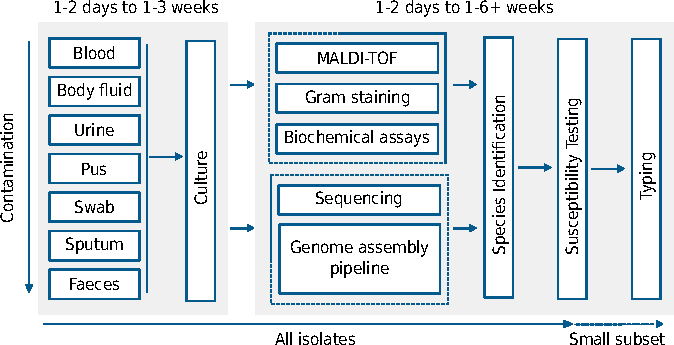
\includegraphics[angle=0,width=\textwidth]{figures/introduction/Figure3.pdf}
    \caption[Schematic representation of the workflow for processing samples of bacterial pathogens.]{Schematic representation of the workflow for processing samples of bacterial pathogens. Samples collected from normally sterile body sites are cultured on a rich medium with the necessary nutrients to support bacterial growth. For more complex samples, such as faeces, which contain multiple bacterial species, selective media are used to favor the growth of the suspected pathogen. The growth of bacterial cultures can take from a day to several weeks depending on the growth requirements of the organism. After successful culture growth, methods such as \ac{MALDI-TOF}, gram staining and other biochemical assays can be used for species determination, followed by susceptibility testing to determine the \ac{AMR} profile. Depending on the species and the context of the infection, a small subset of the samples may be selected for further characterization using typing methods. Typing methods allow for a more detailed characterization of bacterial pathogens, which is especially useful in surveillance and outbreak investigation settings. DNA sequencing technologies are frequently used to substitute or complement phenotypic and molecular assays, allowing detailed characterization of bacterial pathogens through the analysis of the bacterial genomes with specialized bioinformatics methods. DNA sequencing is especially relevant as an alternative to reduce turnaround time when processing fastidious bacteria, for which susceptibility testing through more traditional methods can take from weeks to months. Adapted from \cite{didelot_transforming_2012, mendes_towards_2023}.}
    \label{fig:introduction_figure3}
\end{figure*}

\section{Genotypic methods}

With the introduction of molecular methods for bacterial characterization, the basis for systematics changed. The distinction based on classical phenotypic criteria was complemented or in part replaced by molecular criteria, particularly molecular sequences, because these methods can offer greater resolution, resulting in more precise phylogenetic analyses and diagnostics. Molecular methods can be divided into three main categories: i) \ac{DNA} banding pattern-; ii) \ac{DNA} hybridization-; and iii) \ac{DNA} sequencing-based methods. The first differentiate bacterial strains based on the size and pattern of \ac{DNA} bands/fragments generated by \ac{DNA} amplification or cleavage of genomic \ac{DNA} using restriction enzymes (\acs{RE}s). The second uses techniques such as \ac{DNA} macroarrays and microarrays, which distinguish strains through hybridization to probes complementary to known sequences. The third determine and compare the \ac{DNA} sequence of genomic regions of interest, often determinant for a particular feature, to discriminate bacterial strains based on sequence variation.

\subsection{DNA banding pattern-based methods}

\ac{DNA} banding pattern-based methods, either through amplification by \ac{PCR} or digestion with \acs{RE}s, can provide accurate and quick results and are generalizable for characterizing strains of any bacterial species.

In this category of methods, one that allows to differentiate bacterial strains and has been widely applied in public health is \ac{PFGE}. \ac{PFGE} is an electrophoretic technique that applies alternating electric fields at different angles to separate large \ac{DNA} molecules ($10kb-10Mb$) \cite{schwartz_separation_1984, herschleb_pulsed-field_2007, lopez-canovas_pulsed_2019}. Prior to electrophoretic separation, \acs{RE}s that recognize uncommon motifs are used to cleave the bacterial \ac{DNA}. The distinct banding patterns produced by \ac{PFGE} reflect the \ac{DNA} polymorphisms at the \acs{RE}s recognition sites and, ideally, can be uniquely associated to a specific bacterial strain. The resolution of \ac{PFGE} depends on the choice of the \acs{RE}s used, with \acs{RE}s that recognize long and rare motifs yielding potentially more discriminatory results. The standardization of \ac{PFGE} protocols and the creation of pattern databases, such as the one hosted by Pulsenet International\footnote{\url{https://www.pulsenetinternational.org/protocols/pfge}}, were crucial to the wide adoption of \ac{PFGE}. Although widely used, \ac{PFGE} is laborious and the results can be influenced by multiple factors, which hinders reproducibility and interoperability \cite{li_bacterial_2009}. Due to these limitations and to the invention of \ac{HTS}, \ac{PFGE}, once considered the gold standard for bacterial typing \cite{neoh_pulsed-field_2019}, has gradually been replaced by more accurate and versatile methods based on \ac{WGS}, which allow a much more detailed and increasingly cost-effective characterization of bacterial strains based on the complete or nearly complete genome sequence.

Another method used to differentiate bacterial strains and infer relatedness is \ac{RFLP} \cite{thibodeau_use_1987, todd_chromosome_2001}. \ac{RFLP} allows to differentiate patterns of electrophoresis-separated restriction fragments by Southern Blotting with labeled probes \cite{southern_detection_1975}. The similarity of the patterns of Restriction Fragments (\acs{RF}s) is the basis for strain differentiation. Ribotyping is a variation of \ac{RFLP} that uses probes with conserved domains of \ac{rRNA} genes to differentiate strains based on variable regions flanking the bacterial \ac{rRNA} operons \cite{bingen_use_1994}. The distinct banding patterns identified through this approach are named ribotypes. Since \ac{rRNA} operons are universal, ribotyping is highly applicable. Furthermore, it generates fewer fragments that \ac{RFLP} approaches based on frequently cutting \acs{RE}s, enabling easier interpretation of results and establishment of nomenclature and database systems. The potential cost-effectiveness of \ac{RFLP} can be overturned by time- and labor-consuming protocols, as well as the requirement for large amounts of high-quality \ac{DNA}, which is not always available. Ribotyping is an important method for the characterization and surveillance of \textit{Clostridioides difficile}, with some ribotypes associated with greater disease severity. To overcome the limitations of \ac{RFLP} specifically applied for ribotyping of \textit{C. difficile}, prediction directly from \ac{WGS} data can be performed with bioinformatics methods that estimate sequence similarity, such as sourmash \cite{moore_k-mer_2022, irber_sourmash_2024}, or using machine learning \cite{qi_p-224_2025}.

It would be unacceptable to move to the next category of molecular methods without mentioning the Swiss Army Knife of molecular biology: \ac{PCR}. The \ac{PCR} method, originally developed by Kary Mullis, allows the amplification of any target \ac{DNA} sequence in a sample in a cyclic process to generate a large number of copies of the target sequence \cite{mullis_specific_1986}. \ac{PCR} is performed by temperature cycling, with each cycle having three stages: denaturation, annealing, and elongation. Firstly, high temperature is applied during the denaturation stage to separate the \ac{DNA} strands. Secondly, the temperature is lowered to allow for the annealing of two oligonucleotide primers that flank the target sequence. Lastly, the temperature is raised to the optimum level at which a heat-stable polymerase can extend the primers by incorporating \ac{dNTPs}. Over the years, a plethora of \ac{PCR}-based methods were developed to expand the applicability and overcome limitations of the original \ac{PCR}, firmly establishing \ac{PCR} as one of the fundamental methods in molecular biology.
From the vast number of \ac{PCR}-based methods that were invented, some, such as multiplex \ac{PCR} and \ac{qPCR}, are broadly applicable. Multiplex \ac{PCR} uses multiple primer pairs to simultaneously amplify multiple target sequences in the same \ac{PCR} reaction \cite{chamberlain_deletion_1988}. \ac{qPCR} allows to simultaneously amplify target sequences and detect the \ac{PCR} product \cite{higuchi_simultaneous_1992, kubista_real-time_2006}. This is achieved by incorporating and monitoring the fluorescence of dyes or probes, which increases proportionally to the amount of product formed. \ac{qPCR} overcomes challenges related to product quantification in the original \ac{PCR} and allows for faster confirmation of the presence of a target sequence.
Other \ac{PCR}-based methods were developed for more specific tasks, such as genotyping. Methods such as \ac{AP-PCR or RAPD} \cite{welsh_fingerprinting_1990, williams_dna_1990}, which uses arbitrary primers for random amplification, and \ac{REP-PCR} \cite{versalovic_distribution_1991, de_bruijn_use_1992}, which amplifies regions between interspersed repetitive elements, generate fragment patterns that can function as signatures for specific bacterial strains. The identification of \ac{VNTR} in bacterial genomes through \ac{MLVA} enables to identify polymorphic sites \cite{lindstedt_multiple-locus_2005}. \ac{VNTR} elements evolve rapidly and the number of tandem repeats per locus may vary between strains. \ac{MLVA} uses \ac{PCR} to amplify multiple \ac{VNTR} loci, followed by analysis of the banding pattern to assign a genotype and infer phylogenetic relationships. Although \ac{MLVA} is a simple technique and may offer high resolution, \ac{VNTR} loci in closely related strains may evolve quickly, hindering long-term surveillance. Additionally, \ac{VNTR} may not be common in some species, which limits its applicability, and the accuracy of \ac{MLVA} might be affected by insertions or deletions in the amplified regions.
Some \ac{PCR}-based methods combine \ac{PCR} with other typing methods, such as methods that use \acs{RE}s, to overcome limitations and improve accuracy. One example is \ac{PCR}-\ac{RFLP}, which can amplify target regions directly from clinical or environmental samples and uses \acs{RE}s digestion of the \ac{PCR} amplicons to generate a limited number of \acs{RF}s that are more easily separated by gel electrophoresis and interpreted \cite{wichelhaus_rapid_2001}.
\ac{PCR}-based methods display multiple advantages, such as being relatively inexpensive, fast, and sensitive. Notwithstanding, researchers should be mindful about the inherent limitations of each \ac{PCR}-based method, and of limitations which are common to most \ac{PCR}-based methods, such as the potential for contamination, artifacts caused by, for example, non-specific amplification and primer dimerization, and the need for multiple controls. \ac{PCR} primer design is facilitated by tools such as Primer-BLAST\footnote{\url{https://www.ncbi.nlm.nih.gov/tools/primer-blast/}}, made freely available by the \ac{NCBI} \cite{ye_primer-blast_2012}. Multiple bioinformatics tools\footnote{\url{https://www.gear-genomics.com/silica/}}$^{,}$\footnote{\url{https://bigsdb.readthedocs.io/en/latest/data_analysis/in_silico_pcr.html}}$^{,}$\footnote{\url{https://ucsc.gao-lab.org/cgi-bin/hgPcr}} implement \ac{PCR}-like functionalities to search for sequences of interest based on flanking regions. \textit{In silico} \ac{PCR} is especially valuable to assess primer specificity in a range of applications and to identify highly variable regions whose detection is suboptimal with more common sequence comparison techniques such as alignment \cite{kalendar_silico_2024}.
\ac{PCR} also plays a crucial role in \ac{DNA} sequencing workflows, such as being used for clonal template generation to boost signal detection and the amplification of loci of interest for target sequencing experiments. A brief overview of \ac{DNA} sequencing technologies is presented in Subsection \ref{ssec:introduction_dna_sequencing_technologies}.

\subsection{DNA hybridization-based methods}

\ac{DNA} hybridization-based methods use probes, which correspond to known \ac{DNA} fragments, to detect complementary \ac{DNA} sequences extracted from samples \cite{freeman_fundamentals_2000}. A variant of these methods uses \ac{DNA} arrays to test for the presence of hundreds to tens of thousands of \ac{DNA} fragments, being relevant for applications such as the study of the genetic diversity of bacteria and in transcriptomics. Two types of \ac{DNA} arrays exist: macroarrays \cite{gress_hybridization_1992, lennon_hybridization_1991} and microarrays \cite{derisi_use_1996, schena_quantitative_1995, shalon_dna_1996}. The former can contain up to five thousand spots, providing enough resolution to detect genes involved in \ac{AMR} or for typing methods based on the detection of polymorphisms in a smaller number of loci, such as spoligotyping for \ac{MTC} bacteria. \ac{DNA} microarrays are more expensive, but provide far greater discriminatory power, including up to tens of thousands of distinct probes, enabling the identification of a greater number of loci compared to macroarrays or to study the variation at the genome or transcriptome level. Since the probes included in microarrays are defined based on reference sequences, microarrays may lack probes complementary to accessory genes, leading to an underestimation of genetic diversity. \ac{DNA} microarrays can use \ac{cDNA} or shorter oligonucleotides as probes. The former are used to determine gene presence, while the latter is capable of detecting smaller patterns of variation, such as deletions or even \acp{SNP}. The use of \ac{DNA} arrays has largely been supplanted by the use of \ac{HTS} \cite{bumgarner_dna_2013}.

A \ac{DNA} hybridization-based method that has been applied to overcome some limitations of the classic culture-dependent approach is target capture through hybridization using oligonucleotide probes. In this approach, specialized bioinformatics software is used to design a set of probes to capture bacterial \ac{DNA} directly from clinical samples for subsequent \ac{HTS} \cite{dickson_probe_2021, chafin_mrbait_2018}. Bypassing the culture step is especially useful in reducing the turnaround time for fastidious bacteria such as \textit{M. tuberculosis} \cite{macedo_molecular_2023}, or to capture the \ac{DNA} of uncultivable bacteria, such as \textit{Treponema pallidum}, the causative agent of syphilis \cite{pinto_genome-scale_2016}. In addition, target capture has the potential to provide a less biased view of within-host variation by allowing to capture \ac{DNA} from multiple strains, contrasting with culture-dependent approaches, which may not meet the growth requirements of specific strains and often select a single colony from the culture plate for further characterization. In combination with \ac{HTS}, target capture allows culture-independent sequencing of clinical samples for faster diagnostics and detailed bacterial characterization. Designing probes to capture taxa at multiple taxonomic levels is also a powerful approach to study complex clinical samples and for metagenomics studies, allowing capture of known and related sequences and minimizing the obscuring effect of host \ac{DNA} abundance \cite{dickson_probe_2021}. The success of target capture is highly dependent on multiple factors, such as the specificity of the designed probes, hybridization efficiency, and the abundance of the target microorganisms in the samples \cite{dennis_target-enrichment_2022, macedo_molecular_2023, pinto_genome-scale_2016}.

\subsection{DNA sequencing technologies} \label{ssec:introduction_dna_sequencing_technologies}

The advent of \ac{DNA} sequencing technologies represented a major milestone in biological research, finally unlocking the genetic information encoded in \ac{DNA}, which had already been established as the source of genetic information in 1944 by Oswald Avery while working with \textit{Streptococcus pneumoniae} \cite{avery_studies_1944} and whose three-dimensional structure was determined in 1953 by Watson and Crick based on the crystallographic data produced by Rosalind Franklin and Maurice Wilkins \cite{watson_molecular_1953, zallen_despite_2003}. The potential and continuous improvement of these technologies contributed to their adoption and led to the development of highly reproducible and accurate methods used to differentiate bacterial strains and identify determinants of phenotypic features of interest. As sequencing throughput and sequence data availability increased, the diverse and highly dynamic nature of bacterial genomes was unveiled, leading to an unprecedented interest in developing sequence-based methods that could probe into the accumulated sequence data to gain new insights. The application of \ac{HTS} is revolutionizing our understanding of human health and disease by elucidating fundamental biological and ecological processes.

\subsubsection{First-generation DNA sequencing}

The first major breakthrough in \ac{DNA} sequencing technologies was made by Fredrick Sanger et al. in 1977 \cite{sanger_dna_1977}. Sanger sequencing, also called dideoxy sequencing or chain termination \ac{DNA} sequencing, determines the nucleotide sequence of a single-stranded template \ac{DNA} using a \ac{DNA} polymerase to synthesize nucleotide fragments of different lengths by incorporating radio or fluorescently labeled \ac{ddNTPs} and through premature termination of the \ac{DNA} amplification elongation step \cite{heather_sequence_2016, rodriguez_genesis_2023}. The truncated fragments resulting from the interruption of the elongation step are size-separated by capillary gel electrophoresis to reconstruct the original sequence. As the first successful \ac{DNA} sequencing technology, Sanger sequencing was instrumental in projects such as the sequencing of the first bacterial genome, the genome of \textit{Haemophilus influenzae} \cite{fleischmann_whole-genome_1995}, and the Human Genome Project, which in 2003 achieved the monumental task of determining the first nearly complete sequence of a human genome \cite{international_human_genome_sequencing_consortium_finishing_2004}.
Sanger sequencing was the most widely used sequencing technology until newer and cheaper \ac{HTS} technologies were developed.

\subsubsection{Second-generation DNA sequencing}

The second revolution in \ac{DNA} sequencing began in the early 2000s when the first massive parallel sequencing technologies were made commercially available. Pyrosequencing \cite{nyren_solid_1993, ronaghi_real-time_1996, margulies_genome_2005} was the first second generation \ac{SBS} technology to reach the market (Figure \ref{fig:introduction_figure4}). The general principles of second generation \ac{SBS} technologies are the following: i) attachment of the \ac{DNA} to be sequenced to a solid support, usually combined with amplification to enhance signal detection; ii) single-stranded \ac{DNA} synthesis; iii) primer-dependent incorporation of complementary bases; iv) detection of each incorporated nucleotide for sequence determination. Pyrosequencing is based on real-time quantitative detection of pyrophosphate released as nucleotides are incorporated into a growing \ac{DNA} sequence, yielding reads around 400-500 \ac{bp} long. Initially, libraries of \ac{DNA} molecules are attached to paramagnetic beads via adapter sequences and amplified through emulsion \ac{PCR}. Ideally, on average only one \ac{DNA} molecule attaches to each bead so that each bead is coated in a clonal \ac{DNA} population after emulsion \ac{PCR}.

\begin{figure*}[h!]
    \centering
    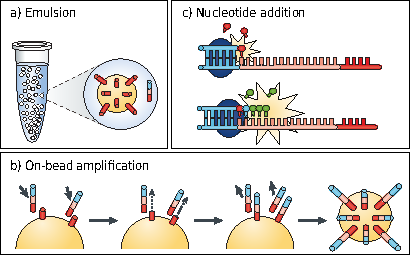
\includegraphics[angle=0,width=\textwidth]{figures/introduction/Figure4.pdf}
    \caption[454 pyrosequencing]{454 pyrosequencing. In 454 pyrosequencing, fragmented DNA templates are amplified through emulsion \ac{PCR} (\textbf{a}), which consists on the hybridization of the DNA templates to bead-bound primers followed by amplification to cover each bead in thousands of copies of the same DNA sequence (\textbf{b}). The beads are arrayed onto a microtitre plate along with primers and different beads that contain enzymes. Sequencing occurs in cycles. In each cycle, a single nucleotide species is added and nucleotides are incorporated into growing chains by a DNA polymerase. When a base is incorporated, the release of an inorganic pyrophosphate triggers an enzyme cascade, resulting in light. Each burst of light is detected by a device to determine the bases incorporated at a particular bead, with the possibility of incorporating multiple bases of the same type in a single cycle (\textbf{c}). Adapted from \cite{loman_twenty_2015, goodwin_coming_2016}.}
    \label{fig:introduction_figure4}
\end{figure*}

The \ac{DNA}-coated beads are distributed into a plate that fits one bead per well where pyrosequencing occurs as bead-linked enzymes and \ac{dNTPs} are added and the pyrophosphate release is detected by a sensor \cite{heather_sequence_2016, nyren_history_2015, ronaghi_sequencing_1998, nyren_enzymatic_1987}. Compared to conventional Sanger sequencing, pyrosequencing has much higher throughput with a fraction of the cost, making it easier and more viable to scale-up. It does have some limitations over Sanger sequencing, however, as the read lengths are shorter, making downstream analysis, such as assembly, more complex. The most used pyrosequencing technology was 454 sequencing, which had major advantages over traditional Sanger sequencing, as demonstrated by its application to investigate drug resistance in \textit{Mycobacterium tuberculosis} \cite{andries_diarylquinoline_2005} and the whole genome sequencing of Jame Watson’s genome in record time and within a fraction of the cost of the Human Genome Project \cite{rothberg_development_2008, wheeler_complete_2008}. 454 sequencing was eventually discontinued in favor of more accurate and advanced technologies, such as Illumina’s \ac{SBS}.
Further improvements to massive parallel \ac{SBS} were introduced with the development of reversible and fluorescently labeled terminators \cite{turcatti_new_2008}. The most widely known sequencing strategy that incorporated these improvements is Illumina’s \ac{SBS} (Figure \ref{fig:introduction_figure5}) \cite{uhlen_sequential_2023, bentley_accurate_2008, fedurco_bta_2006}. Illumina’s \ac{SBS} systems enable \ac{MPS} of small \ac{DNA} fragments, yielding sequencing reads with up to 300 bp. Illumina’s \ac{SBS} technology starts by binding adapter sequences to the \ac{DNA} libraries, which contain complementary sequences that bind to the flow cell, unique indexes or barcodes for sample identification, and the sequencing primer binding sites. The \ac{DNA} molecules attached to the flow cell undergo bridge amplification to generate clonal clusters. Sequencing is performed in cycles by using ‘reversible-terminator’ \ac{dNTPs} and detecting the fluorescence resulting from the incorporation of nucleotides before proceeding to the next cycle. After sequencing the forward strand in this manner, Illumina’s systems are capable of sequencing the reverse strand, generating \ac{PE} data, which significantly improves the accuracy of downstream analysis. The advantages of Illumina’s \ac{SBS} systems, such as their high throughput, lower costs and accurate base calling, led to their worldwide adoption and establishment as the dominant sequencing technology for projects of any scale. The higher throughput of Illumina’s \ac{SBS}, especially as sequencing costs decreased, led to an explosion of sequence data, effectively pushing research into the era of \textit{big data} and data-driven research \cite{uhlen_sequential_2023}. The tremendous increase in the number of microbial genomes deposited in public databases in recent years is in great part due to the widespread application of second-generation sequencing technologies, especially of Illumina’s \ac{SBS}. Other examples of the successful application of this technology are the sequencing of 25,000 cancer genomes by the Cancer Genome Consortium \cite{zhang_international_2019} and the 100,000 Genomes Project \cite{the_100000_genomes_project_pilot_investigators_100000_2021}.

\begin{figure*}[h!]
    \centering
    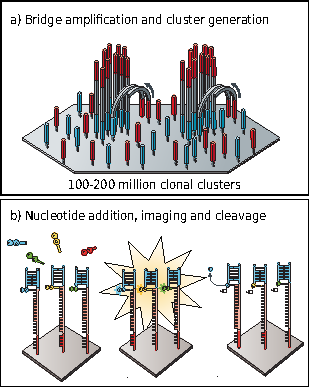
\includegraphics[angle=0,width=0.7\textwidth]{figures/introduction/Figure5.pdf}
    \caption[Illumina's \ac{SBS}]{Illumina's \ac{SBS}. In Illumina's SBS, DNA templates hybridize with adapters bound to a flow cell and are amplified though bridge-PCR to generate millions of clonal clusters (\textbf{a}). In each cycle, fluorophore-labelled and terminally-blocked nucleotides are added and hybridize to complementary bases. Flow cells are imaged to measure the color of the emitted light when a base is incorporated (\textbf{b}). Fluorophores are cleaved and washed before a new cycle begins. Adapted from \cite{loman_twenty_2015, goodwin_coming_2016}.}
    \label{fig:introduction_figure5}
\end{figure*}

\subsubsection{Third-generation DNA sequencing}

Advances in the early 2010s led to the third and current revolution in \ac{DNA} sequencing.
The third-generation of sequencing technologies provide single-molecule sequencing and eliminate the requirement of \ac{DNA} amplification characteristic of second-generation sequencing technologies. Currently, the most successful technologies are HiFi sequencing from \ac{PacBio} \cite{wenger_accurate_2019, eid_real-time_2009} and Nanopore sequencing from \ac{ONT} \cite{mikheyev_first_2014, stoddart_single-nucleotide_2009}. HiFi sequencing (Figure \ref{fig:introduction_figure6}.a) works by creating circularized \ac{DNA} libraries that are sequenced in repeated passes to generate several subreads per \ac{DNA} molecule, which can be compared to determine a consensus read minimizing sequencing errors. HiFi sequencing occurs inside small wells on a \ac{SMRT} Cell microchip where \ac{DNA} extension with fluorescent \ac{dNTPs} is finely monitored. The sequencing technology developed by \ac{ONT} (Figure \ref{fig:introduction_figure6}.b) passes \ac{ssDNA} through a biological nanopore embedded in a synthetic membrane, across which a voltage is applied. The passage of the \ac{ssDNA} through the nanopore limits ionic flow and induces a current change for a period of time that allows to infer the sequence of the \ac{ssDNA} traversing the nanopore. Both technologies generate reads with length that can far exceed the length of the reads generated by second-generation technologies, which is why they are also called long-read technologies. With HiFi sequencing, read lengths can reach 1 to 25 \ac{kb}. Nanopore sequencing is capable of generating even longer reads, from a few to more than a hundred \ac{kb}, and up to several \ac{Mb}. Accuracy-wise, HiFi sequencing has the high ground, but nanopore sequencing provides faster results and greater portability, crucial in outbreak investigation settings for fast pathogen detection and characterization. In addition, the lower entry cost, the development of new nanopores, base calling software, and experimental protocols tailored to particular applications have contributed to a gradual improvement in the accuracy of nanopore sequencing \cite{wang_nanopore_2021, wick_autocycler_2025, foster-nyarko_nanopore-only_2023, wick_trycycler_2021}. Despite continuous improvements in long-read sequencing technologies, their error rate is still higher than that of short-read sequencing technologies, such as Illumina's \ac{SBS}. For this reason, long- and short-read data have been used in combination for so-called hybrid approaches to overcome the limitations of both sequencing technologies and obtain higher-quality genome assemblies. When applied to the assembly of bacterial genomes, this strategy allows to assemble complete and error-free genomes, which cannot be achieved by using any of the technologies separately \cite{wick_assembling_2023, bouras_hybracter_2024, stevens_comparison_2023, wick_assembling_2023, bouras_hybracter_2024}.

\begin{figure*}[h!]
    \centering
    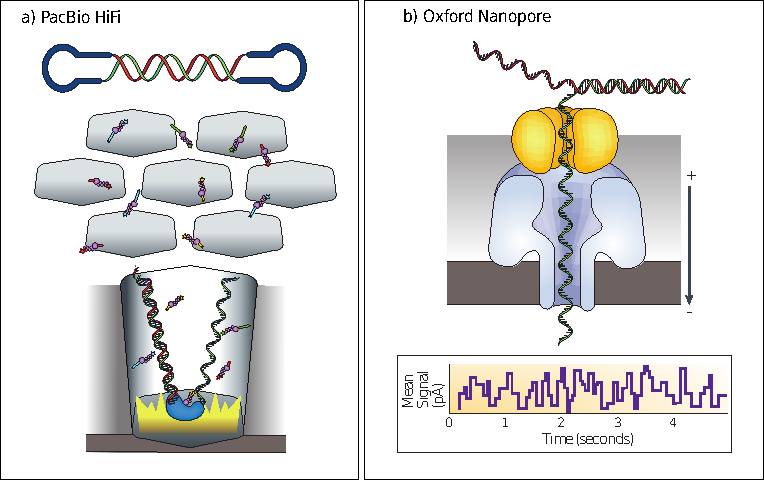
\includegraphics[angle=0,width=\textwidth]{figures/introduction/Figure6.pdf}
    \caption[PacBio HiFi and Oxford Nanopore sequencing]{PacBio HiFi and Oxford Nanopore sequencing. In HiFi sequencing (\textbf{a}), two hairpin adapters are added to the DNA templates to allow for continuous circular sequencing. HiFi sequencing occurs inside wells where labelled dNTPs are incorporated and a camera records the emitted light to determine the incorporated bases. In Nanopore sequencing (\textbf{b}), a leader adapter is bound to the DNA templates and interacts with a motor protein and a biological nanopore, directing the DNA into the pore. As the DNA translocates the pore, a shift in voltage is measured to determine the composition of the DNA sequences. Adapted from \cite{loman_twenty_2015, goodwin_coming_2016, wang_nanopore_2021, metzker_sequencing_2010}.}
    \label{fig:introduction_figure6}
\end{figure*}

\subsection{DNA sequencing-based methods}

As \ac{HTS} technologies became more accurate and cost-effective, wide adoption by research and public health institutions became a possibility. The application of these technologies to help resolve infectious disease events, such as the cholera epidemic in Haiti after the 2010 earthquake \cite{barzilay_cholera_2013} and the international outbreak of \textit{Escherichia coli} disease linked to contaminated fenugreek sprouts \cite{king_outbreak_2012, mellmann_prospective_2011}, quickly revealed that they were an invaluable tool for the surveillance and outbreak investigation of bacterial pathogens. \ac{WGS} of bacterial isolates, performed with second or third generation sequencing technologies, followed by genome assembly, allows the determination of the complete or nearly complete genome sequence, which in principle encodes most of the genetic features necessary for a detailed characterization of an isolate. Genome assembly is performed with pipelines such as Shovill\footnote{\url{https://github.com/tseemann/shovill}}, INNUca\footnote{\url{https://github.com/B-UMMI/INNUca}} \cite{prjibelski_using_2020, walker_pilon_2014, bolger_trimmomatic_2014}, and Bactopia\footnote{\url{https://github.com/bactopia/bactopia}} \cite{petit_bactopia_2020}, typically based on a \textit{de novo} approach to determine a set of contiguous sequences, called \textit{contigs}, resulting from the comparison and combination of overlapping sequencing reads. The application of specialized bioinformatics software allows identifying the relevant features for typing and diagnosis based solely on a sequence approach, complementing or replacing traditional microbiological workflows \cite{besser_next-generation_2018, deurenberg_application_2017}. Moreover, \ac{WGS} may also allow for the identification of emerging genetic features not tested for in routine molecular tests and the detection of uncultivable bacterial strains \cite{deurenberg_application_2017}.

The surveillance of food-borne diseases has greatly benefited from the implementation of standardized \ac{WGS}-based systems. An estimated 600 million people fall ill due to contaminated food annually, resulting in over 400 thousand premature deaths \cite{who_global_2022}. This puts global public health systems under strain and leads to significant costs related to medical treatment and to productivity and trade losses. Initial reports on the adoption of \ac{WGS} by the PulseNet surveillance network in 2000 demonstrated improved outbreak detection and an increase in the number of solved outbreaks compared to using \ac{PFGE} data \cite{besser_next-generation_2018, jackson_implementation_2016, ribot_pulsenet_2019}. The gradual adoption of \ac{WGS} by the network participants and the standardization of analytical workflows established \ac{WGS} as the gold standard for typing of foodborne pathogens tracked by the network. In 2019, the \ac{ECDC} published a strategic framework for the integration of molecular and genomic typing into European surveillance and multi-country outbreak investigation \cite{european_centre_for_disease_prevention_and_control_ecdc_2019}. The document included a progress report on the implementation of \ac{WGS} for surveillance and outbreak investigations by the \ac{EU/EEA} member states and outlined key technological milestones to improve the surveillance and outbreak detection of priority pathogens/diseases. Joint work of the \ac{ECDC} and \ac{EFSA} resulted in the implementation of the \ac{EFSA} and \ac{ECDC} One Health \ac{WGS} System, which aims to augment surveillance capacity and coordination among \ac{EU/EEA} member states \cite{authority_efsa_guidelines_2022}. This system has been instrumental in detecting and resolving multiple multi-country outbreaks \cite{efsa_prolonged_2024, authority_prolonged_2024, european_centre_for_disease_prevention_and_control_european_food_safety_authority_multi-country_2023, european_centre_for_disease_prevention_and_control_european_food_safety_authority_multi-country_2022}.

Building \ac{WGS} capacity requires significant investment in sequencing instruments, reagents, and computational resources to store and analyze \ac{WGS} data. The choice of analytical methods is crucial and may be especially complex as there are multiple fundamental approaches which are not necessarily equivalent or comparable \cite{mixao_multi-country_2025}. Multiple bioinformatics methods have been developed for the detailed characterization of bacterial strains. Some methods characterize strains based on the identification of a single locus, such as \textit{in silico} serotyping or abundance estimation based on the 16S \ac{rRNA} gene. Other methods offer greater resolution by identifying and measuring the variability of a greater number of loci, such as \ac{GbG}, \ac{SNP}-based, and \textit{k}-mer-based methods. These methods have been increasingly integrated into \ac{WGS}-based systems for surveillance, outbreak investigation, and the study of bacterial populations. For this reason and because of their superior potential for further improvement, they are more relevant to the work developed in this dissertation, and a greater focus is given to these methods in the following sections.

\subsubsection{Multilocus sequence typing}

\ac{MLST} is a sequence-based approach that uses allele fragments, typically seven, from housekeeping genes to characterize microorganisms, with a more expressive application for bacterial species of pathogenic potential. \ac{MLST} is based on the principles of \ac{MLEE}, but uses nucleotide sequences at each locus, taking advantage of developments in sequencing technologies and bioinformatics (Figure \ref{fig:introduction_figure7}) \cite{urwin_multi-locus_2003}. Moreover, \ac{MLST} allows identifying a larger number of alleles per locus, offering higher discrimination than \ac{MLEE} while using a smaller number of loci. \ac{MLST} was initially developed to better accommodate vertical and horizontal genetic transfer signals by targeting multiple well-conserved genes and to overcome the challenges of traditional and molecular typing methods, such as the inability to infer strain relatedness and poor reproducibility within and between laboratories \cite{maiden_multilocus_1998}.

\begin{figure*}[h!]
    \centering
    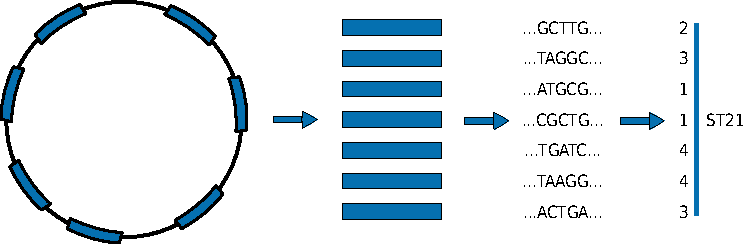
\includegraphics[angle=0,width=\textwidth]{figures/introduction/Figure7.pdf}
    \caption[Multilocus Sequence Typing]{Multilocus Sequence Typing (MLST). In \ac{MLST}, the internal fragments of a set of housekeeping genes, typically seven, are amplified through \ac{PCR} and sequenced. Each distinct sequence is assigned an allele identifier, and the combination of allele identifiers constitutes an allelic profile. Each distinct allelic profile is assigned a \ac{ST}, which allows to identify groups of similar strains.}
    \label{fig:introduction_figure7}
\end{figure*}

The distinct fragments identified at each locus are assigned unique integer identifiers in order of discovery, and the combination of identifiers for the allele fragments identified in all loci constitutes an allelic profile, which can be compared against a database of known allelic profiles. Each distinct allelic profile unambiguously defines a \ac{ST}, assigned to isolates for direct comparisons. \ac{ST}s are grouped into Clonal Complexes (\acs{CC}s), a concept first introduced to describe \textit{Neisseria meningitidis} isolates analyzed by \ac{MLEE}, based on their similarity to a central \ac{ST} (allelic profile or genotype). The definition of central \ac{ST}s is achieved through a combination of computational and experimental data obtained from public health authorities. Newly identified \ac{ST}s are assigned to the most similar \acs{CC} based on a minimum number of shared alleles with the central \ac{ST}. \ac{ST} organization into \acs{CC}s facilitates epidemiological analysis, often grouping most \ac{ST}s into a much smaller number of \acs{CC}s and allowing to identify \acs{CC}s of greater clinical relevance. One disadvantage of \ac{MLST} is that it may not offer the same degree of discrimination within lineages or species with highly conserved housekeeping genes. Furthermore, due to the diversity of bacterial species, \ac{MLST} schemes must be developed to distinguish closely related bacteria, usually at the genus and species levels, or they may not provide sufficient resolution. Consequently, \ac{MLST} cannot be applied as a combined taxonomic and typing approach at all levels of bacterial diversity \cite{jolley_ribosomal_2012}.

By relying on the sequencing of allele fragments from multiple chromosomal locations, \ac{MLST} provides unambiguous results and is more robust to recombination events, constituting a faster and more sensitive technique than most laborious lab protocols, which also tend to be more unpredictable as variation accumulates. Since allele fragments are used as a unit of comparison, single allele differences constitute a single event, regardless of the number of nucleotide polymorphisms involved. While this model may not provide resolution for every single point change, it is resistant to horizontal genetic transfer events, which introduce a lot of variation in a single event, leading to an inaccurate estimate of similarity if counted as multiple differences.

\ac{MLST} aims to provide good discrimination for short- and long-term epidemiology. The original study showed that it was congruent and more discriminatory than \ac{MLEE} in distinguishing hyper-virulent strains of \textit{N. meningitidis} while also offering a clear distinction between lineages at the species level \cite{enright_multilocus_1999}. A subsequent study presented a \ac{MLST} database for \textit{Streptococcus pneumoniae}, obtaining consistent results with \ac{MLEE} and \ac{PFGE} for the analysis of predominantly invasive and antibiotic-resistant isolates \cite{enright_multilocus_1998}. Moreover, \ac{MLST} was also congruent with serotyping, with isolates that share the same or similar \ac{ST}s also expressing the same serotype, except for cases where recombination at the capsular locus was suspected to have led to capsular switching \cite{enright_multilocus_1999}.

Numerous \ac{MLST} databases have been developed since \ac{MLST} was proposed. Currently, a public collection of curated and frequently updated \ac{MLST} databases is available for a great number of microbial species on the PubMLST website\footnote{\url{https://pubmlst.org/}}. PubMLST integrates sequence data with sample metadata to promote the exchange of molecular typing data for epidemiological studies. As of 27 March 2025, PubMLST manages more than 130 species and genera-specific \ac{MLST} databases, which contain tens of millions of alleles identified and submitted by researchers. The sheer volume of data and the range of databases in PubMLST highlight how the advantages of \ac{MLST} contributed to its rapid adoption worldwide, with the technique widely used for epidemiological studies, to identify localized disease outbreaks and monitor local and global trends, and for population studies, to examine the structure of bacterial populations and perform evolutionary analyzes.

\subsubsection{rMLST}

Greater resolution and wider applicability than \ac{MLST} are achieved with \ac{rMLST}. \ac{rMLST} typing indexes the variation of the genes encoding the bacterial \ac{rps}. The \ac{rps} genes are ideal targets for universal bacterial characterization because they are: i) universally present; ii) distributed across the genome, which makes \ac{rMLST} more robust against horizontal gene transfer events that reassort loci and break phylogenetic congruence; and iii) encode proteins which are functionally conserved across the Bacteria domain. \ac{rMLST} constitutes a combined taxonomic and typing approach for the whole domain of Bacteria at all taxonomic levels. \ac{rMLST} allelic profiles or \acp{rST} determined through \ac{rMLST} provide a basis for universal bacterial systematics, allowing for a precise identification of the phylogenetic position at any taxonomic rank, while also distinguishing closely-related strains for typing purposes. A database for the 53 \ac{rps} genes identified in bacteria is managed by the \ac{BIGSdb} platform \cite{maiden_mlst_2013}.

\subsubsection{wg/cgMLST}

The level of resolution for typing depends on the desired application. On the one hand, higher resolution is necessary for the detection of outbreaks and within-patient variation. On the other hand, lower resolution is required to group strains into \acs{CC}s or lineages. The \ac{GbG} approach is inherently hierarchical and scalable, meaning that the number of genes used in the analyzes can be adjusted based on the desired resolution \cite{maiden_mlst_2013}. Thus, the concept and analysis methods of the highly successful seven-gene \ac{MLST} can be intuitively scaled to hundreds or thousands of genes to encompass diversity at the core- or whole-genome level, giving rise to \ac{wg/cgMLST} (Figure \ref{fig:introduction_figure8}). \ac{wg/cgMLST} provides higher resolution for surveillance and outbreak investigation. Furthermore, the additive nature of \ac{MLST}, through the continuous update of schemas with novel alleles, ensures that \ac{wg/cgMLST} can provide accurate results in the long-term while also promoting interoperability.

\begin{figure*}[h!]
    \centering
    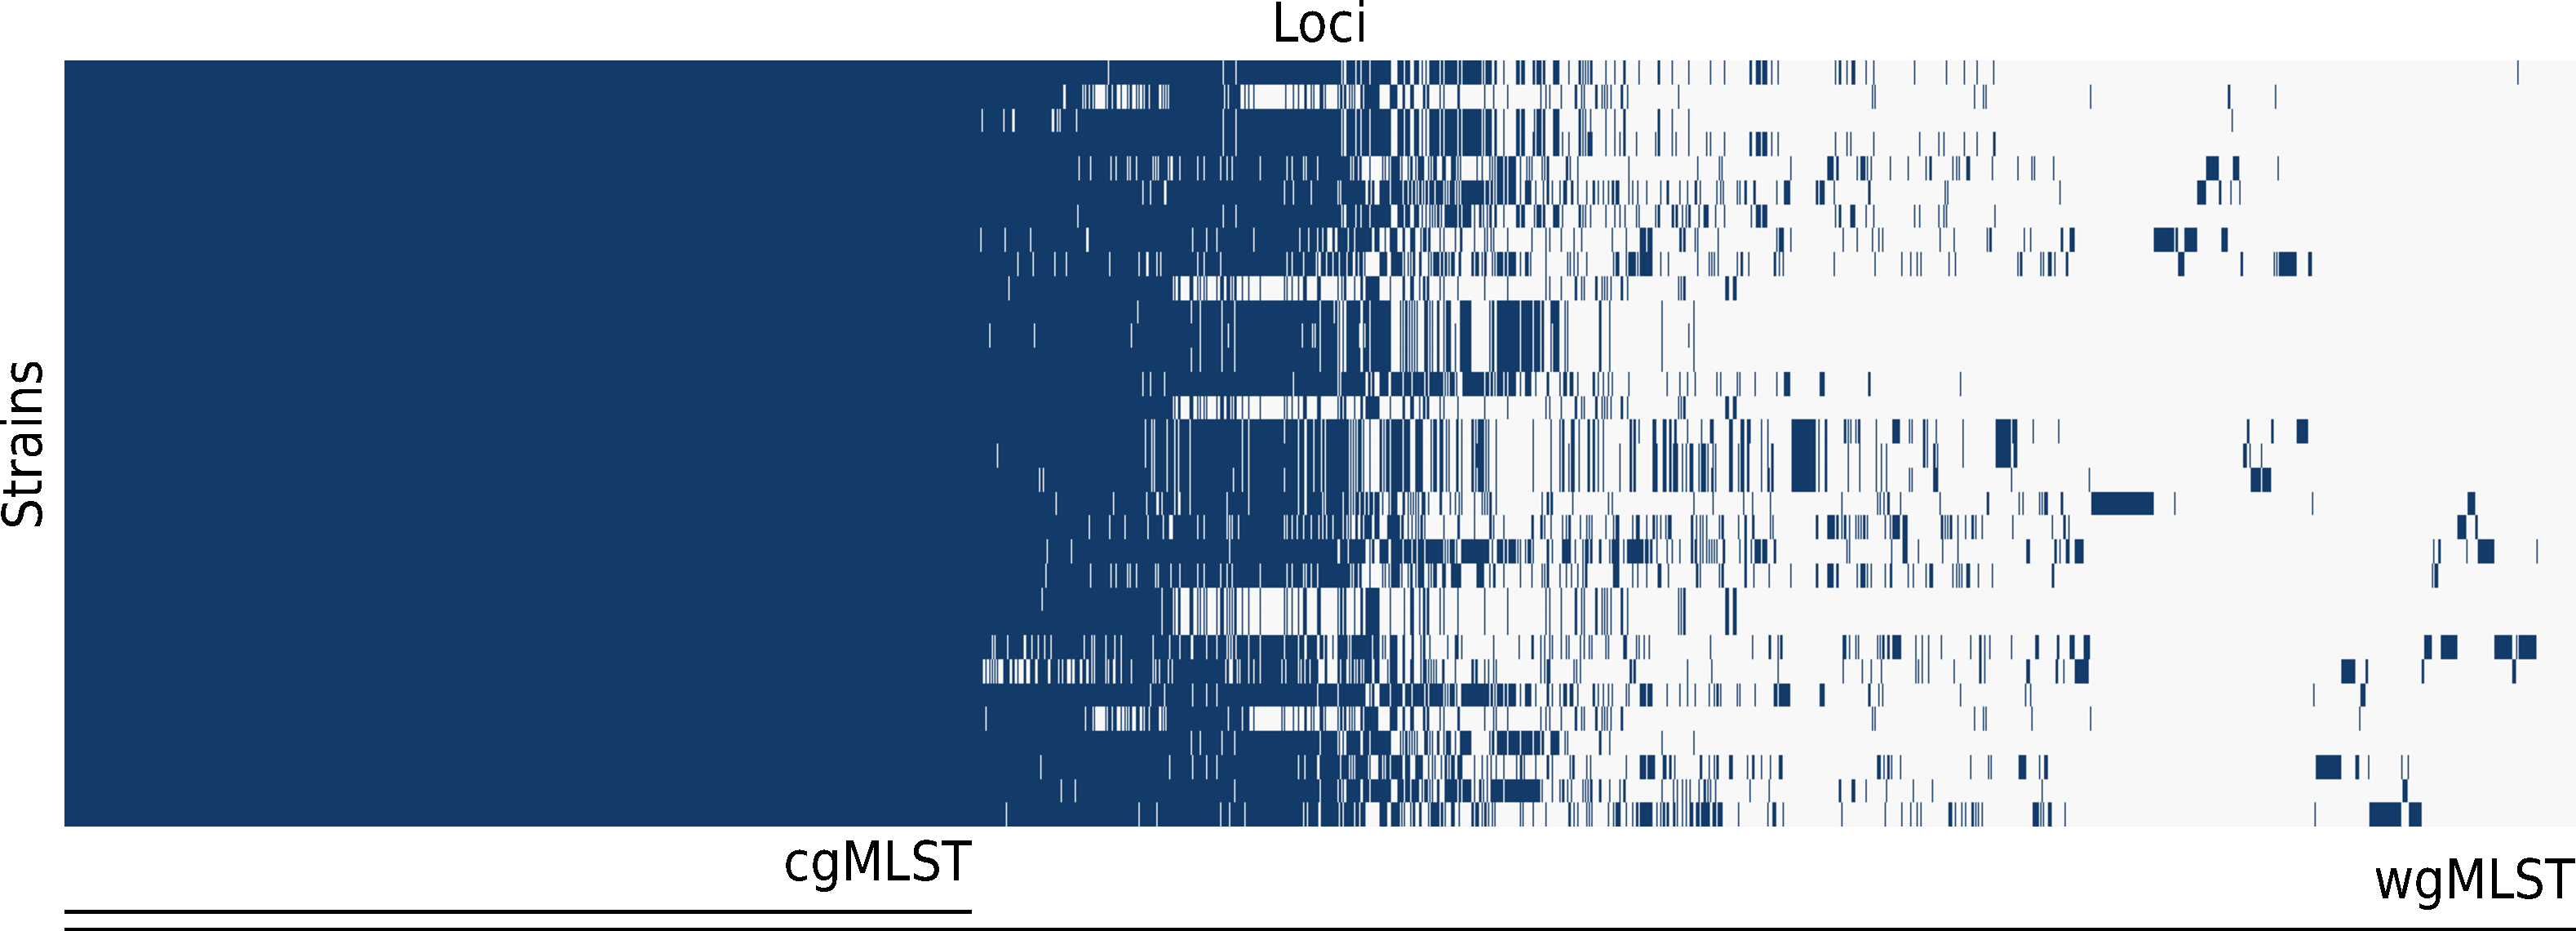
\includegraphics[angle=0,width=\textwidth]{figures/introduction/Figure8.pdf}
    \caption[Whole- and core-genome MLST]{Whole- and core-genome \ac{MLST} (\ac{wg/cgMLST}). The heatmap represents a presence-absence matrix of the loci (columns) in a wgMLST schema that were identified in 32 bacterial strains (rows). Darker regions indicate that a locus was identified in a strain, while lighter regions indicate locus absence. \ac{cgMLST} compares the set of alleles for the loci present in all strains (shorter line below the heatmap), while \ac{wgMLST} incorporates loci from the accessory genome (longer line below the heatmap), providing greater resolution.}
    \label{fig:introduction_figure8}
\end{figure*}

\ac{cgMLST} characterizes bacterial strains based on the identification and comparison of the genes that constitute the core genome. Although the core genome is often defined as the set of genes present in all strains of a given dataset, a more relaxed definition is needed to account for technical and biological variation. A loci presence threshold of 95\% is commonly used to accommodate biases and errors introduced by, for example, the sequencing and genome assembly processes. This allows to retain genes that are present in almost all strains of a species or that are reported as absent due to misassembly. Furthermore, the set of core loci is usually determined based on the allele calling results for a specific dataset ideally representative of the diversity of the species. This means that the definition of core genome is highly dependent on the dataset used and the number of core loci detected varies according to the species and the dataset.

\ac{wgMLST} further expands the set of loci used for strain typing by including loci from the accessory genome. The frequency of accessory loci is highly variable, with some accessory loci being nearly as frequent as core loci, and others being found only in a small subset of strains or even being strain-specific. In theory, a \ac{wgMLST} schema should contain more loci than a \ac{cgMLST} schema, but there are no hard requirements regarding the fraction of core and accessory loci of a species that should be included, allowing for \ac{wgMLST} schemas with a number of loci close to that of a \ac{cgMLST} schema or considerably larger \ac{wgMLST} schemas encompassing all known core and accessory loci for a species. Since \ac{wgMLST} identifies more loci than \ac{cgMLST}, it provides greater resolution and is potentially more discriminatory when there is variation in the accessory genome. However, creating \ac{wgMLST} schemas requires a more careful selection of target loci compared to \ac{cgMLST} schemas. While \ac{cgMLST} schemas include only core loci, which usually display lower allele diversity, the inclusion of accessory loci in \ac{wgMLST} schemas increases the frequency of spurious loci due to sequencing and assembly errors or real sequence variability, affecting the accuracy of the results. Since \ac{cgMLST} provides robust results and most of the available schemas are \ac{cgMLST} schemas, most analyses are performed at that level, with \ac{wgMLST} being recommended when higher resolution is necessary, such as when comparing closely related strains for surveillance and outbreak detection \cite{mixao_multi-country_2025, joseph_evaluation_2023, leeper_evaluation_2023, leeper_validation_2025}.

\ac{wg/cgMLST} characterizes strains by determining their allelic profiles (i.e., the set of loci and alleles identified in each strain). The comparison of the allelic profiles to determine the number of shared loci and alleles provides an estimate of strain similarity. This can be done by discarding missing loci from the analysis or by computing the absolute difference. The former is preferred, as genome fragmentation and potential sequencing and assembly errors make it impossible to be certain if a locus that was not identified is in fact absent from the genome. The cross-comparison of a set of samples allows to compute a distance matrix including the number of allelic differences between each pair of strains. The distance matrix enables phylogenetic analysis through methods such as single-linkage clustering, \ac{NJ} or by computing a \ac{MST}. Computing a \ac{MST} is frequently used in surveillance and outbreak investigation scenarios as it provides accurate results when comparing closely related strains. For the study of more diverse populations, more robust results can be obtained using methods such as maximum likelihood after computing a \ac{MSA} for the alleles identified in all strains for each locus and concatenating the loci \ac{MSA}a to obtain a core genome \ac{MSA}. Multiple software and web platforms provide functionalities to generate and visualize trees from \ac{wg/cgMLST} results, including options to overlay the tree with metadata to more easily identify relevant strains. A distance threshold can be defined to identify groups of highly similar strains corresponding to lineages or potential outbreaks. Threshold definition is often empirical, depending on the diversity of the species, dataset, context, and methods used for the analysis. Consequently, threshold values are not universally applicable, which hinders comparability of the results obtained in different settings (e.g., outbreak detection in different countries.

\paragraph{wg/cgMLST platforms} \mbox{}\\

There are multiple web platforms that store and manage \ac{wg/cgMLST} schemas. These platforms provide access to \ac{wg/cgMLST} schemas for a wide range of species and offer different functionalities for data analysis. All well-established \ac{wg/cgMLST} platforms centralize data analysis by requiring users to upload their data. Platforms such as \ac{BIGSdb}\footnote{\url{https://pubmlst.org/software/bigsdb}} and Enterobase\footnote{\url{https://enterobase.warwick.ac.uk/}} operate under more permissive licenses, providing wide-access to schemas and functionalities upon registration and allowing other users or institutions to set up their own instances of the platform. Other platforms, such as Ridom SeqShere+\footnote{\url{https://www.ridom.de/seqsphere/}}, are proprietary software that requires users to pay for access to the platform's functionalities, although schemas used within the platform are publicly available. The results generated within different platforms are not directly comparable, as schemas for the same species stored by different platforms may target different sets of loci and use distinct loci and allele nomenclatures, which hinders interoperability. The results are not easily comparable even when the schemas have the same origin and use the same nomenclature, since each platform applies different methods for allele identification and the nomenclatures are not synchronized, which means that different identifiers can be assigned to the same allele depending on the platform.

\ac{BIGSdb} was the first platform to enable \ac{wg/cgMLST} and is a prime example of a solution for \ac{wg/cgMLST} that has been widely adopted and offers extensive analytical capabilities. \ac{BIGSdb} extended the functionalities for \ac{MLST} of the PubMLST platform to \ac{WGS} data \cite{jolley_bigsdb_2010, jolley_open-access_2018}. \ac{BIGSdb} pioneered the application of \ac{GbG} methods to genome analysis, storing genomic and gene sequences, as well as associated metadata, such as provenance and phenotypic data for isolates from which the sequence data originated. Additionally, it stores allele and locus definitions, without an inherent limit to the number of records or the number of schemas into which the loci can be grouped. The loci included in a schema do not need to be associated with a single organism, enabling the creation of schemas that encompass the diversity of genes, such as accessory genes, that are distributed in diverse organisms. Known and novel alleles are identified from sequence data uploaded to \ac{BIGSdb} to maintain a record of the known diversity of genes identified in the samples stored in the database. Furthermore, genomic data are periodically rescanned as the database expands to identify variants in stored isolates that could not be detected previously based on the represented allele diversity in the database. The functionalities included in \ac{BIGSdb} allow users to link isolate and sequence data with great flexibility, allowing the definition of schemas encompassing the diversity of species with utility for epidemiological investigations and population analysis or smaller schemas to study particular aspects of the biology of an organism. The genetic nomenclatures established and maintained by \ac{BIGSdb} enable the definition of classification hierarchies for an effective comparison of bacterial isolates globally \cite{jolley_open-access_2018}.

\subsubsection{SNP-based methods}

An accurate estimation of strain similarity for phylogenetic analyzes can be achieved by comparing the genomes of strains of interest against the genome of a reference strain to identify \acp{SNP}. This is performed by mapping sequencing reads against a reference genome to identify all variable positions in regions shared with the reference, identifying the set of core \acp{SNP} (Figure \ref{fig:introduction_figure9}). Similarly to \ac{wg/cgMLST}, pairwise \ac{SNP} distances or the alignment of the core \acp{SNP} can be determined to perform phylogenetic analysis with methods such \ac{NJ} or maximum likelihood, respectively. Since \ac{SNP}-based approaches identify variation at the single nucleotide level, they can potentially provide higher resolution than \ac{wg/cgMLST} for the regions being considered. However, it is necessary to meet two requirements for high-resolution typing with \ac{SNP}-based methods. First, choosing a reference genome closely related to the strains under investigation is of the utmost importance, as \acp{SNP} are only identified in the regions shared with the reference. A more divergent strain may considerably reduce the number of shared regions, and consequently the number of detected \acp{SNP}. Strategies for choosing a reference genome include selecting a high quality genome from the same \ac{ST}, \acs{CC}, serogroup or determining the genome distance to a group of candidate reference genomes to select the most appropriate. Second, the group of strains under investigation cannot be very diverse, as that will also reduce the number of regions considered for \ac{SNP} determination \cite{jolley_bigsdb_2010}. These requirements can be met for outbreak detection and investigation scenarios in which \ac{SNP}-based methods have been successfully applied to resolve national and international outbreaks. However, these requirements limit the applicability of \ac{SNP}-based methods compared to \ac{wg/cgMLST} approaches, which can be used to characterize from very diverse datasets to closely related strains. In addition, \ac{SNP}-based methods are less robust to recombination and \ac{HGT} than \ac{wg/cgMLST}, as a single event will lead to the identification of multiple \acp{SNP}, potentially overestimating the distance between strains. The congruence between \ac{SNP}-based and \ac{wg/cgMLST} approaches is highly dependent on the reference genome and the schema used, respectively, as well as the parameters used and the dataset under analysis. While some studies have reported good congruence between both approaches for outbreak analyses, others have highlighted that the results are not directly comparable and that a congruence analysis is necessary to assess method equivalence \cite{mixao_multi-country_2025}. Furthermore, \ac{SNP}-based approaches do not scale as well as \ac{wg/cgMLST}, in part because they are more computationally demanding as the size of the dataset increases, but also because it may be necessary to use multiple references and fine-tune the parameters for accurate \ac{SNP} detection, making it harder to standardize or establish a reference database for consistent results. Nevertheless, variant calling data can be stored to promote reproducibility and minimize scalability concerns, an approach implemented in SnapperDB \cite{dallman_snapperdb_2018}.

\begin{figure*}[h!]
    \centering
    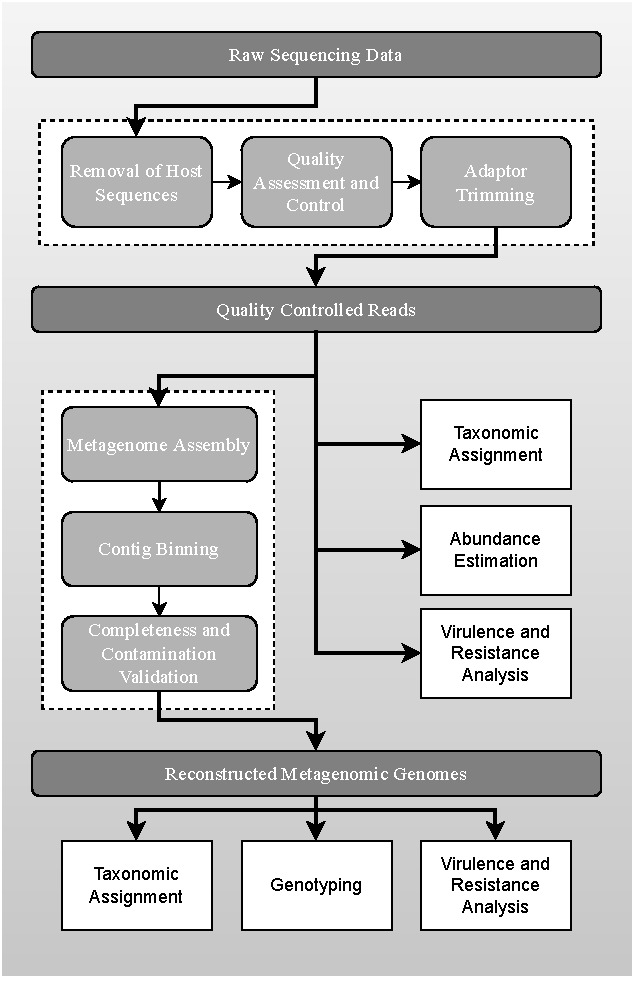
\includegraphics[angle=0,width=\textwidth]{figures/introduction/Figure9.pdf}
    \caption[SNP-based methods]{SNP-based methods map the sequencing reads or genome assemblies from bacterial strains against a reference genome to identify \acp{SNP}. The top sequence in the image represents a region of the reference genome and the bottom lines represent the same region for a group of strains compared against the reference. The positions that differ from the reference genome are colored in red.}
    \label{fig:introduction_figure9}
\end{figure*}

\subsubsection{\textit{k}-mer-based methods}

Although the concept of \textit{k}-mer has existed for several decades, even if under different designations (e.g., N-gram, k-tuple, w-mers), its wide application to increase the efficiency and accuracy of bioinformatics methods is relatively recent. \textit{k}-mer-based approaches break sequences into smaller subsequences of length \textit{k} (Figure \ref{fig:introduction_figure10}). This seemingly simple approach of \textit{break it to understand it} has enormous potential, allowing for much more time-efficient sequence comparisons than alignment-based approaches. However, storing large sets of \textit{k}-mers in memory can lead to high memory usage. Thus, it is important to optimize parameters such as the \textit{k}-mer size and sampling method, also termed sketching (i.e., which \textit{k}-mers to select from all possible \textit{k}-mers generated from a sequence). With respect to \textit{k}-mer size, it is important to optimize it for the desired application by balancing the trade-off between greater specificity achieved with longer \textit{k}-mers and greater sensitivity with shorter \textit{k}-mers. Optimizing \textit{k}-mer selection is more complex and has been the subject of extensive research \cite{roberts_reducing_2004, sahlin_effective_2021, ndiaye_when_2024, karami_designing_2024, kille_minmers_2023, shaw_theory_2022}.

\begin{figure*}[h!]
    \centering
    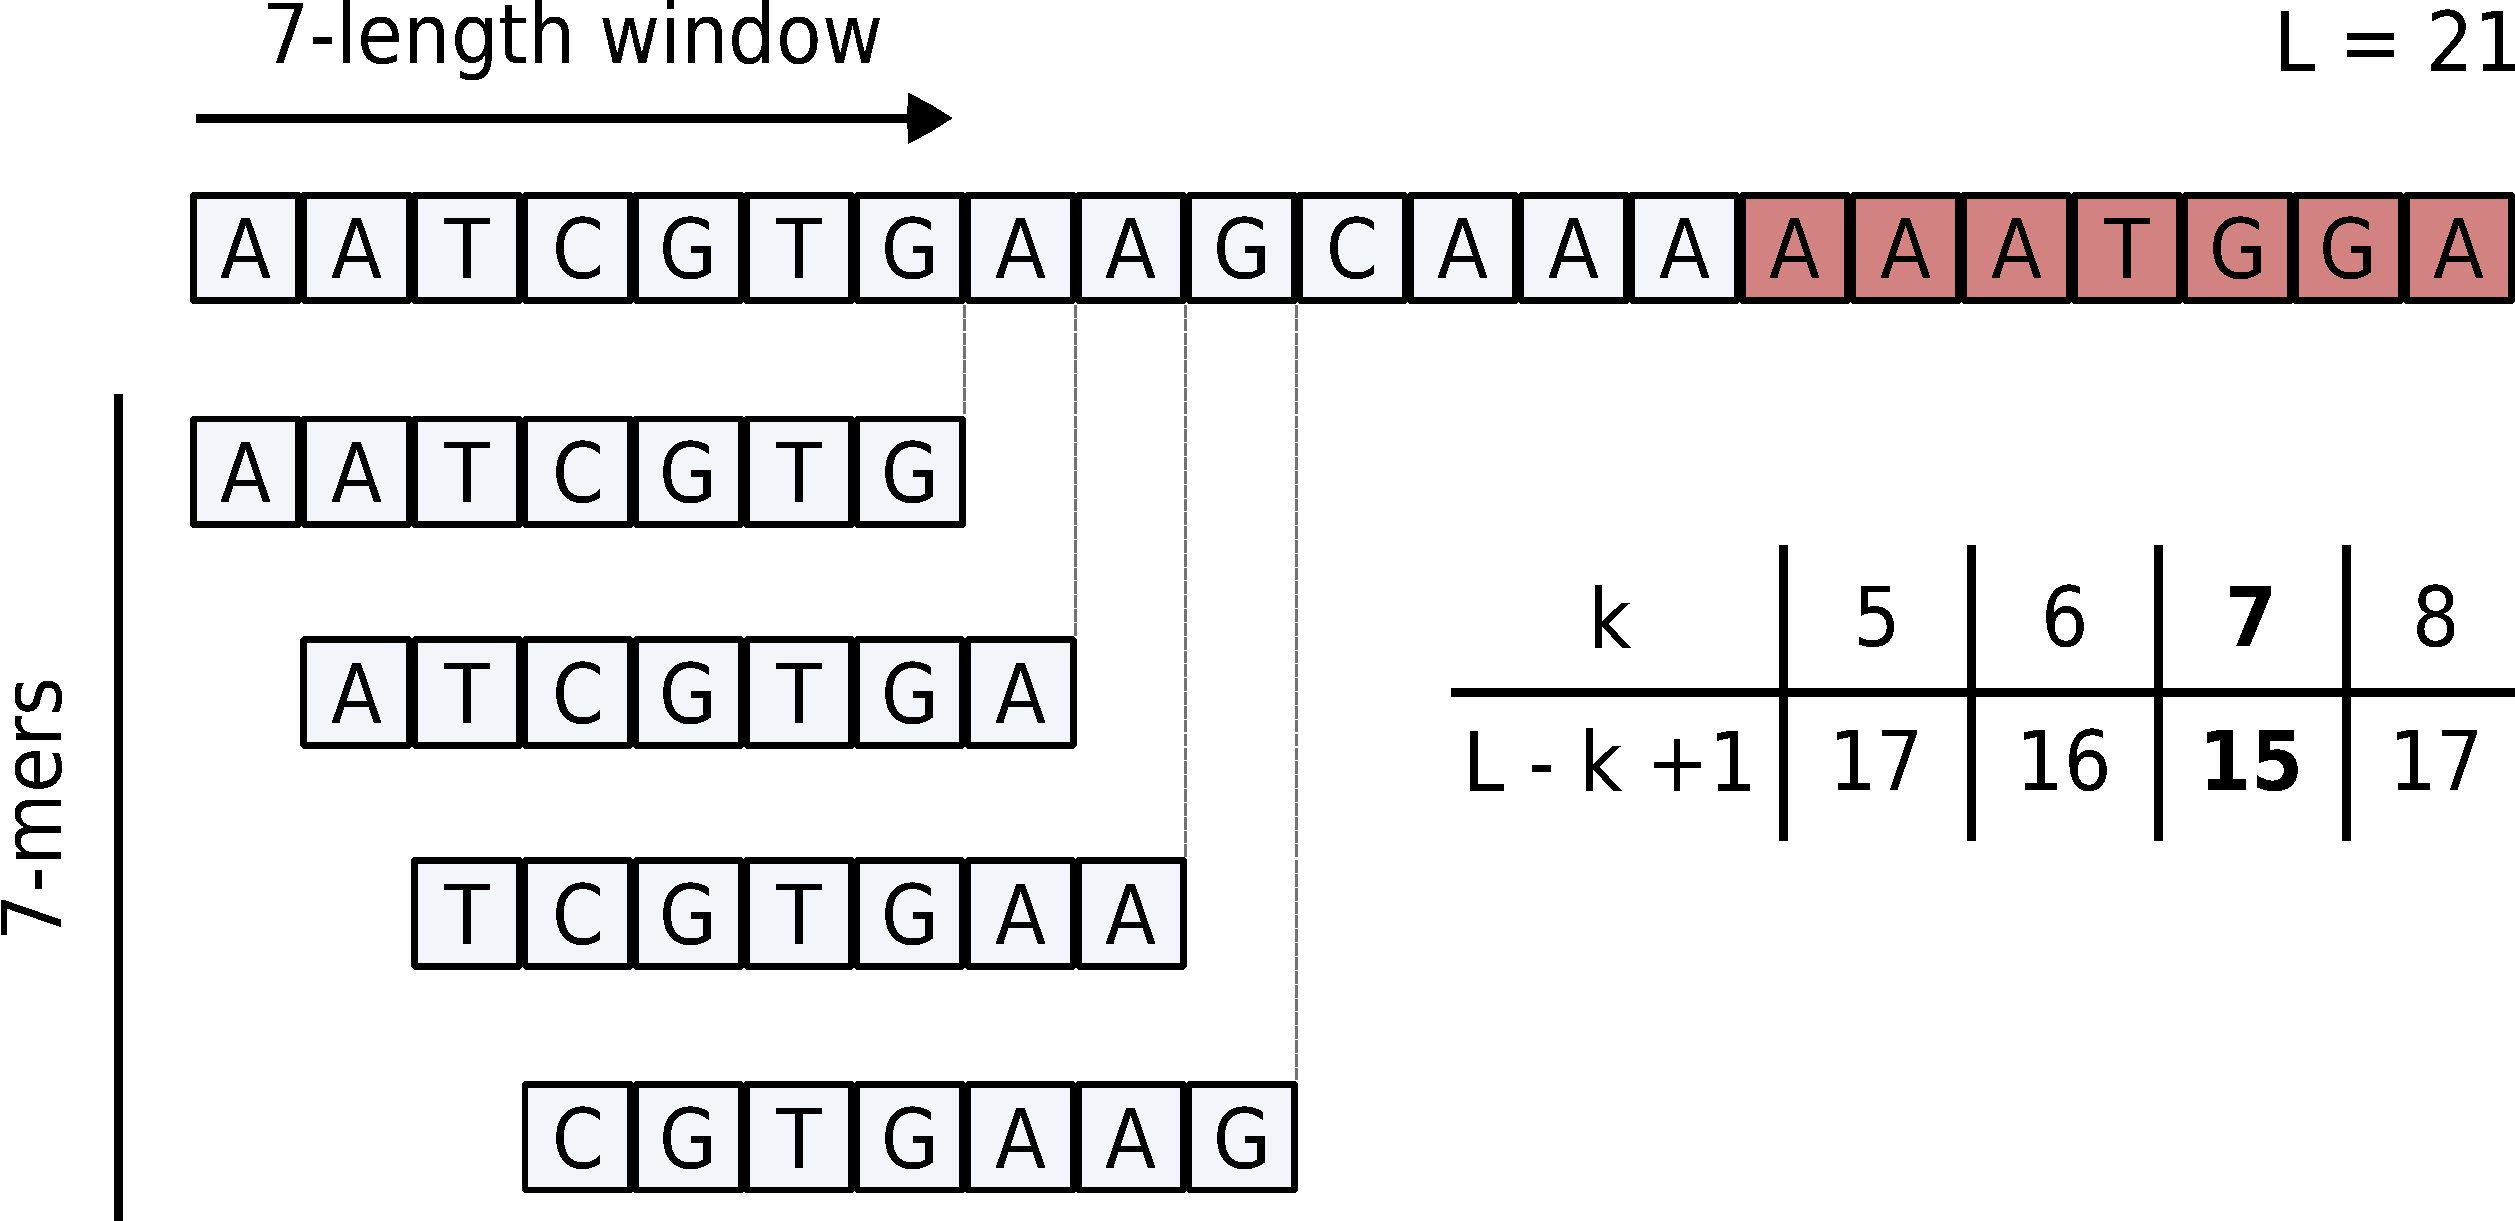
\includegraphics[angle=0,width=\textwidth]{figures/introduction/Figure10.pdf}
    \caption[Determining \textit{k}-mers]{Determining \textit{k}-mers. After defining the value of \textit{k}, the first \textit{k}-mer is determined by selecting the segment with the first \textit{k} bases in the sequence. The next \textit{k}-mer is determined by sliding one position to the right to select a new \textit{k}-mer that differs from the first one by a single position. This process is repeated until all consecutive \textit{k}-mers for a sequence are determined. The figure represents the determination of 7-mers from a sequence with 21 nucleotides (L). The first four 7-mers are shown below the sequence. The last 7-mer is highlighted in red. The table shows the total number of \textit{k}-mers that can be determined from the sequence by varying the value of \textit{k} from 5 to 8. The column corresponding to the total number of 7-mers is in bold.}
    \label{fig:introduction_figure10}
\end{figure*}

Ideally, it is desired to select the smallest set of \textit{k}-mers that minimizes memory usage without sacrificing accuracy. However, depending on the application, it may be necessary to satisfy other requirements that complicate the determination of the optimal sampling method. For example, a sampling method that selects \textit{k}-mers randomly may be preferred for unbiased sequence comparisons, while optimizing the interval between consecutively selected \textit{k}-mers may offer better performance when sequence variability is higher. Theoretical and empirical evaluations of the performance of each sampling method are important to determine optimal parameters and limitations. Minimizers and spaced seeds are two sampling methods that have been widely applied due to their simplicity and effectiveness in a wide range of applications, such as genome assembly and taxonomic classification. \textit{k}-mers are a centerpiece of most genome assemblers, with the construction of \textit{de Brujin} graphs, representing the overlap between \textit{k}-mers determined from sequencing reads, being the fundamental strategy used by many genome assemblers to solve the problem of genome assembly for both short- and long-read data \cite{medvedev_what_2021}. For taxonomic classification, sequence data are often decomposed into \textit{k}-mers and compared against \textit{k}-mer indexes constructed from taxonomically annotated reference sequences. This strategy allows for ultra-fast taxonomic classification. Kraken was one of the first highly successful \textit{k}-mer based tools for taxonomic classification \cite{wood_kraken_2014}. Its first version enabled fast taxonomic classification based on a minimizer index, and the second version optimized the database structure to reduce memory requirements and added spaced seeds for greater accuracy \cite{wood_improved_2019}. In theory, \textit{k}-mer-based methods offer several advantages over \ac{wg/cgMLST} and \ac{SNP}-based methods. Firstly, there is no need to define a reference database, such as a schema, or select a reference genome to compare strains against. This overcomes the reference bias limitation of \ac{SNP}-based approaches and eliminates the need to store and manage a schema with a specific allelic nomenclature. However, to achieve consistent results, especially when trying to establish a cluster nomenclature, it is still recommended to create a database structure to compare and classify strains. Otherwise, the results obtained for different datasets may not be comparable. Secondly, and contrary to \ac{wg/cgMLST}, \textit{k}-mer-based methods can include non-coding regions to estimate strain similarity. Lastly, if adequately parameterized, \textit{k}-mer-based methods can be faster and more efficient than \ac{wg/cgMLST} or \ac{SNP}-based methods. A good example of an efficient and versatile \textit{k}-mer-based method applicable to closely related samples and outbreak investigation is SKA2 \cite{derelle_seamless_2024}. SKA2 uses split \textit{k}-mer analysis for reference-free and reference-based mapping to genotype bacterial strains using sequencing reads or genome assemblies. Another \textit{k}-mer based tool, PopPUNK \cite{lees_fast_2019}, uses \textit{k}-mers to calculate core and accessory distances, which in turn are used by machine learning algorithms to cluster bacterial strains. This approach has proved useful for population analysis, and the ability to update existing clusters with new strains without having to recalculate all pairwise distances is especially useful for surveillance.

\section{Aims of the Thesis}

The advances in \ac{DNA} sequencing technologies have allowed research and public health institutions to gradually switch from classical and more laborious microbiological workflows to \ac{WGS}-based methods for the characterization of bacterial pathogens. With modern sequencing technologies, it is possible to streamline the genome sequencing of dozens of bacterial strains. The widespread adoption of \ac{WGS} and the increased availability of bacterial genomes in public databases enabled researchers to develop and apply more advanced bioinformatics methods to gain greater insight into the structure, diversity and dynamics of bacterial genomes. \ac{GbG}, \ac{SNP}-based and \textit{k}-mer-based methods allow for a more detailed characterization of bacterial pathogens and are currently widely applied for surveillance, outbreak investigation, and to study the diversity of bacterial species. \ac{GbG} methods in particular, such as \ac{wg/cgMLST}, have been adopted more frequently for surveillance and outbreak investigation, perhaps in part because they constitute an expansion of the classical seven-gene \ac{MLST}, making it conceptually and technically easier to implement and transition to. The wide adoption of \ac{wg/cgMLST} makes it relevant to explore ways in which it can be further improved. The main objective of this work is to explore concepts and implement solutions that improve the efficiency, accuracy, and interoperability of \ac{wg/cgMLST}. The main goals are the following:

- Optimize the processes of schema creation and allele calling in \ac{wg/cgMLST}, as well as implement solutions for comprehensive analysis of the schema and results data;

- Implement a Nomenclature Server to store and manage \ac{wg/cgMLST} schemas that enables local and private analyzes based on a common allelic nomenclature;

- Identify and propose solutions for common problems found during the creation and application of \ac{wg/cgMLST} schemas, either derived from low-quality data or from limitations of current methodologies used in \ac{wg/cgMLST}.

The first goal will be achieved mainly through the optimization of the chewBBACA software for \ac{wg/cgMLST} \cite{silva_chewbbaca_2018}. The second goal will focus on creating a Web service that provides easy access to \ac{wg/cgMLST} schemas and minimizes scalability and data privacy concerns compared to other well-known \ac{wg/cgMLST} platforms that centralize data analysis and require users to share their data. The last goal will help create strategies to identify and correct spurious loci added to \ac{wg/cgMLST} schemas, improve the integration of accessory loci into \ac{wgMLST} schemas, and provide valuable information to guide the development of chewBBACA.
